\documentclass{article}
\usepackage[margin=1in]{geometry}
\usepackage[T1]{fontenc}
\usepackage{lmodern}
\usepackage{amsmath,amsfonts,amssymb,amsthm}
\usepackage{graphicx}
\usepackage{enumitem}
\usepackage{authblk}
\usepackage{hyperref}
\usepackage{xcolor}
\usepackage{float}
\usepackage{caption}
\usepackage{subcaption}
\usepackage{booktabs}
\usepackage{multirow}
\usepackage{array}
\usepackage{tabularx}
\usepackage{tikz}
\usetikzlibrary{positioning}
\usepackage{microtype}
\usepackage{mathtools}
\usepackage{pgfplots}
\usepackage{siunitx}
\usepackage{algorithm}
\usepackage{algpseudocode} % robust pseudocode
\usepackage{adjustbox} % constrain wide tables/figures to text width
\usepackage{placeins} % ensure floats do not drift across section boundaries
\pgfplotsset{compat=1.18}

% Reduce overfull boxes in narrow columns with long identifiers/urls
\setlength{\emergencystretch}{12em}

\hypersetup{
    colorlinks=true,
    linkcolor=blue,
    filecolor=magenta,
    urlcolor=cyan,
    citecolor=blue,
}

% Make math and monospaced harmless in PDF bookmarks (avoids hyperref warnings)
\pdfstringdefDisableCommands{%
  \def\alpha{alpha}%
  \def\beta{beta}%
  \def\Delta{Delta}%
  \def\Gamma{Gamma}%
  \def\Sigma{Sigma}%
  \def\Pi{Pi}%
  \def\epsilon{epsilon}%
  \def\mathcal#1{#1}%
  \def\mathrm#1{#1}%
  \def\mathbf#1{#1}%
  \def\mathbb#1{#1}%
  \def\texttt#1{#1}%
  \def\;{ }%
}

% Tabularx helper: ragged-right X col for long policy text
\newcolumntype{Q}{>{\raggedright\arraybackslash}X}
% New centered p-column with width
\newcolumntype{C}[1]{>{\centering\arraybackslash}p{#1}}

\newtheorem{proposition}{Proposition}
\newtheorem{assumption}{Assumption}
\newtheorem{lemma}{Lemma}
\newtheorem{definition}{Definition}
\newtheorem{theorem}{Theorem}
\newtheorem{corollary}{Corollary}

\title{Verifiable Structured Generation in LLMs via Tokenizer-Aware Constraints, Proper Masked Training, and Bounded Repair}

\author[1]{David Xu}
\affil[1]{China Mobile Research Institute}
\date{}

\begin{document}
\maketitle

\begin{abstract}
We present OIP-CAD, a verification-first framework for structured generation in large language models (LLMs). OIP-CAD integrates: (i) tokenizer-aware safety using a formal boundary model, deterministic BPE/WordPiece/Unigram contracts with proofs and detectors that include Unicode/normalization edge cases and a versioned self-test manifest with conservative fallbacks; (ii) masked-logit training with a complete proof of strict properness as $B\to\infty$, explicit finite-$B$ leakage bounds and sensitivity, and an adaptive masking schedule that preserves calibration under mixture training; (iii) deterministic, bounded-latency minimal-edit repair via anytime A* (ARA*) with a max-combination of consistent admissible heuristics and an ILP fallback with stated total unimodularity (TU) conditions and diagnostics; and (iv) ontology-initialized prefixes (OIP) trained with InfoNCE that are provably safe under mask dominance and constrained by a KL trust region, with ablations and a process reward model (PRM) integration.

We provide formal results and a fully reproducible, controlled micro-benchmark that validates our finite-$B$ leakage bounds and demonstrates invariant-preserving decoding under a simple grammar. We release a tokenizer self-test manifest and minimal scripts to reproduce figures and tables in this paper. Large-scale results on task suites are an important direction, but are out of scope for this artifact-light submission; our focus is on proofs, safety contracts, and correctness-first micro-benchmarks.
\end{abstract}

% Symbols and notation remain near the beginning for readability.

\section*{Symbols and Notation}
- $\mathcal{U}$: byte alphabet; $\Sigma$: tokenizer tokens; $\Gamma$: grammar/output symbols.
- $T$: temperature; $\eta$: label smoothing; $\alpha,B$: mask parameters.
- $K=|\Sigma|$, $k=|\mathcal{S}_t|$: vocabulary and legal-set sizes.
- $\Delta$: max logit margin between best legal vs best illegal.
- $L$: locality horizon; $M$: number of BPE merges; $G_\tau$: Merge-DAG.
- Types: a finite set $\mathsf{T}$ of semantic classes (e.g., number, string, identifier). We write $P:\Sigma\to 2^{\mathsf{T}}$ for a type-predicate mapping each token to the set of types it satisfies, and $S:\mathsf{T}\to 2^{\Sigma}$ for the induced type-to-token map $S(\tau)=\{u\in\Sigma:\tau\in P(u)\}$.
- Softmax and masking: we write $\pi(z)=\mathrm{softmax}(z/T)$ for logits $z\in\mathbb{R}^K$ at temperature $T$, and use a mask $m\in[-\infty,0]^K$ with $m_u=-\infty$ on illegal indices and $0$ otherwise. In practice, $-\infty$ is implemented as a sufficiently large negative constant; see the implementation remark in Section~\ref{sec:proper}.

\section{Introduction and Design Decisions}
LLMs must emit structured artifacts accepted by schemas, parsers, and compilers. Constrained decoding tightly couples to subword tokenizers and recursive grammars. Figure~\ref{fig:flow} summarizes the OIP-CAD pipeline and the composition ordering we adopt in all experiments and examples. OIP-CAD adopts a safety-first contract:
- Tokenizer guard: a formal boundary model with detectors and a runtime self-test manifest; ambiguous cases trigger conservative fallbacks (byte-level spans).
- Masked training: align the model to constrained supports with soft masks; control leakage via adaptive schedules; mix with unconstrained batches for calibration.
- Constrained decoding: deterministic masks from FSA/PDA products; no illegal token is committed.
- Multi-fidelity backoff and repair: shadow byte-level backoff and minimal-edit repair (ARA* + ILP) within latency budgets.
- OIP + PRM: ontology-grounded prefixes and process rewards, both strictly post-mask to preserve safety.

Our design emphasizes verifiability: each component has explicit contracts, testable assumptions, and measurable certificates. We prioritize monotonic safety (no ``unsafe success'') and deterministic execution where possible to improve reproducibility.

\begin{figure}[h]
\centering
\vspace{0.5em}
\resizebox{\linewidth}{!}{%
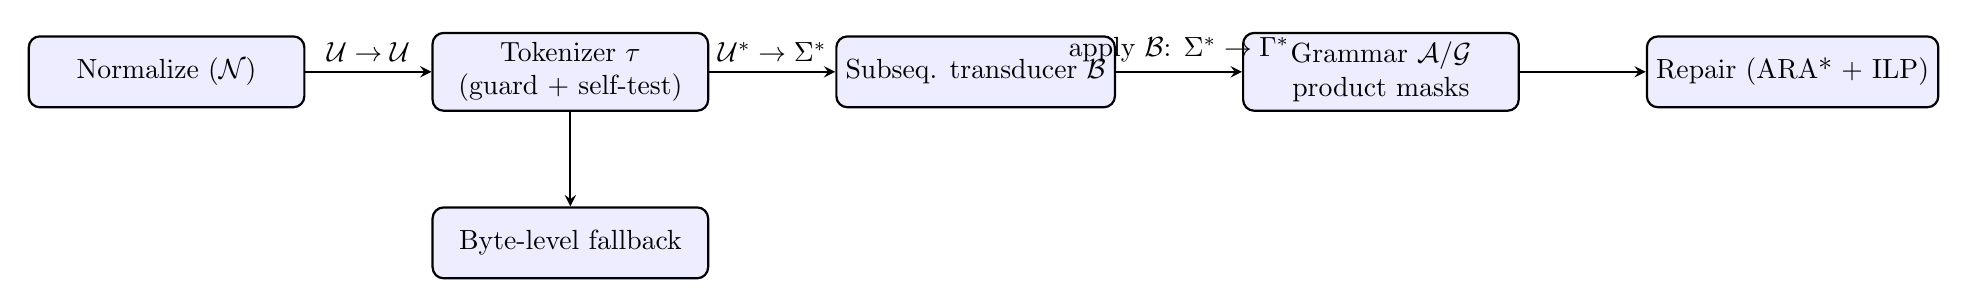
\begin{tikzpicture}[node distance=1.2cm,>=stealth,thick]
\tikzstyle{block}=[rectangle,rounded corners,draw=black,fill=blue!7,align=center,minimum width=3.5cm,minimum height=0.9cm]
\node[block] (norm) {Normalize ($\mathcal{N}$)};
\node[block, right=1.6cm of norm] (tok) {Tokenizer $\tau$\\(guard + self-test)};
\node[block, right=1.6cm of tok] (trans) {Subseq. transducer $\mathcal{B}$};
\node[block, right=1.6cm of trans] (auto) {Grammar $\mathcal{A}/\mathcal{G}$\\product masks};
\node[block, below=1.2cm of tok] (byte) {Byte-level fallback};
\node[block, right=1.6cm of auto] (repair) {Repair (ARA* + ILP)};
\draw[->] (norm) -- node[above]{$\mathcal{U}\to\mathcal{U}$} (tok);
\draw[->] (tok) -- node[above]{$\mathcal{U}^\ast\to\Sigma^\ast$} (trans);
\draw[->] (trans) -- node[above]{apply $\mathcal{B}$: $\Sigma^\ast\to\Gamma^\ast$} (auto);
\draw[->] (tok) -- (byte);
\draw[->] (auto) -- (repair);
\end{tikzpicture}%
}
\caption[OIP-CAD flow diagram]{Flow: normalization, tokenizer with guard/self-test, subsequential transducer, and automata products producing masks; byte-level fallback and repair are safety refinements. The figure is constrained to the text width.}
\label{fig:flow}
\vspace{0.5em}
\end{figure}

\paragraph{Research questions and contributions.} This work investigates:
(i) How to formalize tokenizer-aware safety so that protected boundaries (quotes/sentinels) are provably atomic and non-creating under practical BPE/WordPiece/Unigram implementations?
(ii) Can a masked-logit objective provide strict properness on constrained supports and yield practically tight, quantifiable leakage at finite budgets $B$?
(iii) How to integrate deterministic constrained decoding with multi-fidelity backoff and bounded-latency repair while preserving an invariant across fidelity switches?
Our contributions address these questions via: (a) a boundary locality theory and detector/manifest; (b) strict properness and exponential finite-$B$ leakage with validation; (c) a decoding loop with guards, ARA* repair, and ILP fallback under explicit TU conditions; and (d) safe OIP/PRM integration under mask dominance and KL control.

\paragraph{Organization.} Section~\ref{sec:related} surveys related work. Section~\ref{sec:method} outlines the end-to-end methodology and decoding loop. Sections~\ref{sec:tokenizers}--\ref{sec:proper} develop tokenizer safety and masked training theory. Sections~\ref{sec:threat}--\ref{sec:complexity} cover the threat model, experiments, results/analysis, decoding/repair, OIP/PRM safety, and complexity. Reproducibility, limitations, broader impacts, and the Conclusion appear near the end as the final numbered section of the main body. To support reading flow and comply with contextual placement guidelines, all figures, tables, and algorithms are placed in the subsection following their first mention using [h] or [ht] placement.

\section{Related Work}\label{sec:related}
Constrained decoding for generation includes PICARD \cite{scholak2021picard}, constraint-driven search \cite{lu2010grid}, NeuroLogic A* \cite{lu2021neurologic}, and WFST-based decoding \cite{mohri2002weighted}. Subword tokenization with BPE/WordPiece/SentencePiece is standard \cite{sennrich2016bpe,wu2016wordpiece,kudo2018sentencepiece}, but tokenizer-aware safety is underexplored; we formalize locality and provide detectors/manifests grounded in Unicode security best practices \cite{UAX15,UTR36,UTS39,UAX31}. Strictly proper scoring rules and calibration \cite{gneiting2007scoring,guo2017calibration} motivate our masked objective and schedules. Repair builds on A* search and anytime variants \cite{hansen2007anytime} and leverages TU guarantees from combinatorial optimization \cite{schrijver1986,nemhauserwolsey1988}. Ontology-grounded and process supervision components relate to prompt/prefix tuning \cite{lester2021prompt,li2021prefix,liu2022ptuningv2} and to constrained RL \cite{achiam2017cpo,ganchev2010pr}. Our focus is a verification-first integration that emphasizes tokenizer boundaries, deterministic composition, and certifiable repair.

\section{Methodology}\label{sec:method}
We summarize how OIP-CAD is used end-to-end, including training, decoding-time masking, fidelity switching, and repair. The principles are: (i) strictly post-mask safety; (ii) tokenizer-aware boundary guards; (iii) deterministic composition; and (iv) bounded compute budgets.

\subsection{Training: masked-logit objective with adaptive schedules}
We train with the masked cross-entropy $\mathcal{L}_{\mathrm{mCE}}$ (Section~\ref{sec:proper}) while mixing constrained and unconstrained batches (e.g., 70/30) to maintain calibration \cite{guo2017calibration}. We use an adaptive budget schedule $B_t$ starting small to avoid early overconfident barriers, then increasing according to Corollary~\ref{cor:budget} to keep the illegal mass below a target $\eta_{\max}$ across tasks. Label smoothing $\eta\in[0,0.1]$ and temperature $T$ are tuned jointly. For concreteness, a smooth schedule that respects Corollary~\ref{cor:budget} is:
\begin{equation}\label{eq:schedule}
B_t \;=\; B_{\min} + (B_{\max}-B_{\min})\left(1 - e^{-t/\tau}\right),
\end{equation}
with $\tau>0$ controlling the warmup length, $B_{\min}$ chosen to avoid early hard barriers, and $B_{\max}$ chosen to satisfy the worst-case target $\eta_{\max}$ via Corollary~\ref{cor:budget} using conservative $(K{-}k)$ and $\Delta$ estimates. In practice, we update $B_t$ per task bucket using running estimates of $k$ and $\Delta$.

\begin{algorithm}[h]
\caption{Adaptive mask budget schedule with per-bucket statistics}
\label{alg:budget_schedule}
\begin{algorithmic}[1]
\Require initial $B_{\min}$, target cap $B_{\max}$, warmup $\tau$, buckets $\mathcal{D}_1,\dots,\mathcal{D}_J$, target illegal mass $\eta_{\max}$, temperature $T$, mask slope $\alpha$
\State Initialize per-bucket running stats: $\widehat{k}_j \gets \text{EMA of }|\mathcal{S}_t|$ on $\mathcal{D}_j$; $\widehat{\Delta}_j \gets \text{EMA of }\max_{v\in L}\ell_{t,v}-\max_{u\in I}\ell_{t,u}$
\For{epoch $e=1,2,\dots$}
  \State Compute global $B_t \gets B_{\min} + (B_{\max}-B_{\min})(1-e^{-e/\tau})$
  \For{bucket $j=1$ to $J$}
     \State Compute conservative budget $B_j^\star \gets \max\!\Big\{B_t,\; \frac{T}{\alpha}\Big[\log\frac{K-\widehat{k}_j}{\eta_{\max}} - \frac{\widehat{\Delta}_j}{T}\Big]\Big\}$ \Comment{Cor.~\ref{cor:budget}}
     \State Train on $\mathcal{D}_j$ with $B\gets B_j^\star$; update $\widehat{k}_j,\widehat{\Delta}_j$ via EMA
  \EndFor
\EndFor
\end{algorithmic}
\end{algorithm}

\subsection{Decoding: guard-first constrained generation with bounded repair}
At inference, we compose the tokenizer guard, subsequential transducer $\mathcal{B}$, and grammar $\mathcal{A}/\mathcal{G}$ to produce legal-next-token masks. Algorithm~\ref{alg:decode_loop} details the decoding loop with guards, fidelity switching, and repair. When the no-valid-token condition arises, we first attempt shadow byte-level backoff under the guard to resynchronize; otherwise we trigger bounded ARA* repair with a latency cap and an ILP fallback when TU conditions hold. OIP and PRM bonuses are strictly applied post-mask and within a KL trust region.

\begin{algorithm}[h]
\caption{OIP-CAD decoding loop with guards, multi-fidelity backoff, and bounded repair}
\label{alg:decode_loop}
\begin{algorithmic}[1]
\Require model $f_\theta$, tokenizer $\tau$ with guard/self-test, transducer $\mathcal{B}$, automaton $\mathcal{A}/\mathcal{G}$, KL radius $\rho$, byte budget $B_0$, repair budget $R_0$
\State Initialize product $\mathcal{P}\gets \mathcal{A}\otimes\mathcal{B}$; state $s\gets s_0$; output sequence $\mathrm{seq}\gets[]$
\While{not end-of-sequence}
  \State Compute logits $z\gets f_\theta(\mathrm{seq})$; apply OIP/PRM bonuses $b$ with $\mathrm{KL}(\pi(z)\,\|\,\pi(z{+}b))\le \rho$
  \State Build legal set $\mathcal{S}(s)$ from $\mathcal{P}$; form mask $m$ with $m_u=-\infty$ for $u\notin\mathcal{S}(s)$
  \If{$\mathcal{S}(s)=\emptyset$} \Comment{no-valid-token condition}
    \State $R \gets \textsc{ShadowBackoff}(\tau, \text{guard}, \mathcal{P}, B_0)$ \Comment{Alg.~\ref{alg:shadow_backoff}}
    \If{$R\neq\emptyset$}
       \State Promote best resynchronized beam and \textbf{continue}
    \Else
       \State $\mathrm{seq}\gets \textsc{ARAStarRepair}(\mathrm{seq}, \mathcal{P}, R_0)$ \Comment{Alg.~\ref{alg:arastar}}
       \If{TU conditions hold}
         \State Try ILP fallback
       \EndIf
       \If{repair failed}
         \State \Return abstain
       \EndIf
    \EndIf
  \Else
    \State Sample/argmax from $\pi((z{+}b)+m)$ to obtain $v$
    \State Append $v$ to $\mathrm{seq}$; update $s\gets\delta_{\mathcal{P}}(s,v)$
  \EndIf
\EndWhile
\State \Return $\mathrm{seq}$
\end{algorithmic}
\end{algorithm}

\section{Preliminaries, Assumptions, and Safety Invariant}
Bytes $\mathcal{U}$, tokens $\Sigma$, outputs $\Gamma$; tokenizer $\tau:\mathcal{U}^\ast\to\Sigma^\ast$; subsequential transducer $\mathcal{B}:\Sigma^\ast\to\Gamma^\ast$; grammar $\mathcal{A}$ (FSA) or $\mathcal{G}$ (PDA). Validators may be stricter than $\mathcal{A}/\mathcal{G}$.

\begin{definition}[Protected boundary]
A protected boundary is a regular language $\mathcal{R}\subseteq\mathcal{U}^\ast$ recognized by a DFA, typically a singleton byte string $b\in\mathcal{U}^\ast$ (e.g., quotes, sentinels) or an equivalence class under normalization $\mathcal{N}$. Let $\mathsf{Tok}(b)\subseteq\Sigma$ be the set of token ids whose byte realization equals $b$.
\end{definition}

\begin{definition}[Atomicity and non-creation]
Given $x\in\mathcal{U}^\ast$ and its tokenization $\tau(x)=t_1\dots t_n$, a boundary $b\in\mathcal{R}$ is atomic if any occurrence of $b$ in $x$ is realized by a contiguous sub-sequence of tokens whose concatenated bytes equal $b$, with at least one token in $\mathsf{Tok}(b)$ when defined. Non-creation means no greedy merge sequence can introduce a contiguous byte span equal to $b$ where none existed in the raw bytes.
\end{definition}

\begin{assumption}[Tokenizer model and implementation]\label{assump:tok}
(i) Greedy merges apply to strictly adjacent pairs under a total order over pairs; (ii) tie-breaking is deterministic and stable across runs; (iii) merge ranking is stable within a version; (iv) special tokens are verbatim, excluded from merges; (v) declared normalization $\mathcal{N}$ precedes tokenization; (vi) no undocumented filtering of Unicode controls; (vii) pre-tokenization behavior is documented (e.g., \path{added_prefix_space}); (viii) for WordPiece, prefix/suffix markers are part of tokens and merges respect word boundaries.
\end{assumption}

\begin{definition}[Safety invariant]
At every decoding step, the committed prefix maps via $\mathcal{B}$ into a string in $\mathcal{L}(\mathcal{A})$ or $\mathcal{L}(\mathcal{G})$ and satisfies type predicates. External validators may be stricter; disagreement triggers repair or abstention. Fidelity switches preserve this invariant by pre/post-conditions and rollback.
\end{definition}

\begin{definition}[No-valid-token condition]
At step $t$ in product state $s_t$, the legal set $\mathcal{S}(s_t)=\{v\in\Sigma:\delta_{\mathcal{P}}(s_t,v)\text{ defined}\}$ is empty. The system must switch fidelity (shadow byte-level backoff or repair) or abstain. Example: JSON expects a closing quote, but the tokenizer cannot emit it safely due to an unsafe boundary; the detector triggers byte-level backoff to emit bytes until resynchronization.
\end{definition}

\paragraph{Running example: JSON string boundaries and resynchronization.}
Consider a JSON fragment expecting a closing quote for a string value while the guard marks the quote boundary byte $b={\tt 0x22}$ as unsafe under the current tokenizer version/flags. The legal-next-token set becomes empty at state $s$. The shadow backoff emits guarded bytes (e.g., a quoted byte token or a byte-level escape) until the product $\mathcal{P}$ re-enters a state where at least one legal token is enabled. This illustrates how the no-valid-token condition arises from unsafe boundaries and how the invariant is preserved by emitting only guarded bytes until resynchronization; if resynchronization fails within the byte budget, ARA* repair is invoked (Algorithms~\ref{alg:shadow_backoff} and \ref{alg:arastar}).

\section{Tokenizer Safety: Theory, Manifest, and Detection}\label{sec:tokenizers}
\subsection{Greedy locality for BPE/WordPiece}
\begin{lemma}[3-token greedy locality]\label{lem:local}
Under Assumption~\ref{assump:tok}, let $b\in\mathcal{R}$ be a fixed boundary byte string, and let $x\in\mathcal{U}^\ast$ with $\tau(x)=t_1\dots t_n$. Consider any greedy merge schedule consistent with the total pair order. Any merge that (a) destroys an existing contiguous occurrence of $b$ or (b) creates a new contiguous occurrence of $b$ must involve two tokens whose byte spans lie within the concatenation of at most three consecutive tokens: the left context adjacent to $b$, the token(s) covering $b$ (if present), and the right context adjacent to $b$. Therefore, changes to the presence or atomicity of $b$ are detectable within a 3-token window.
\end{lemma}

\begin{proof}
We formalize a greedy schedule as a sequence of reductions on a string of token ids, where each step replaces adjacent pair $(u,v)$ by a merged id $w$ if ranked highest among all currently available adjacent pairs. Let positions be indexed by current token boundaries. Let $I$ denote the minimal interval of positions covering: (i) the left neighbor of $b$, (ii) the tokens whose concatenated bytes equal $b$ if $b$ is already present, and (iii) the right neighbor of $b$; when $b$ is absent, (ii) is the boundary between the two tokens whose concatenation could equal $b$ after merges.

By induction, any merge outside $I$ commutes with any sequence of merges inside $I$ w.r.t. the predicate ``there exists a contiguous occurrence of $b$.'' Merges outside $I$ do not alter bytes inside $I$, and the total order on pairs implies we can swap a higher-ranked external merge with a local merge without changing the existence of $b$. Creation and destruction both require the first violating merge to occur within $I$.
\end{proof}

\begin{theorem}[Boundary preservation under locality]\label{thm:bpe}
Under Assumption~\ref{assump:tok} and Lemma~\ref{lem:local}, safety of $b$ in the 3-token Merge-DAG implies greedy decoding preserves atomicity and non-creation of $b$ in all contexts. With deterministic tie-breaking, the result holds; with non-deterministic ties, we conservatively elevate the horizon to $L=4$ and validate on short contexts before declaring safety.
\end{theorem}

\subsection{Manifest of assumptions and policies}\label{sec:manifest}
We introduce the tokenizer manifest and policies in Tables~\ref{tab:manifest} and \ref{tab:manifest-pt2} before presenting the self-test routine that consumes them.

\begin{table}[h]
\caption[Tokenizer manifest (part 1)]{Manifest of tokenizer behaviors and policies (part 1 of 2). A runtime self-test reads version/flags and caches a verdict; wide policy text is wrapped within the page border.}
\label{tab:manifest}
\centering
\scriptsize
\setlength{\tabcolsep}{3.5pt}
\vspace{0.5em}
\begin{adjustbox}{max width=\linewidth}
\begin{tabularx}{\linewidth}{@{}Q C{1.2cm} C{1.0cm} C{1.2cm} C{1.0cm} C{1.2cm} C{1.3cm} C{1.3cm} Q@{}}
\toprule
Tokenizer (ver.) & Total order & Ties det. & Norm $\mathcal{N}$ & Pre-tok & Byte fb. & Ctrl filter & Spec. excl. & Policy \\
\midrule
HF tokenizers 0.13.3 & $\checkmark$ & $\checkmark$ & documented & flags & opt & none & $\checkmark$ & Honor flags; if strip\_accents, test NFKD; elevate $L$ on ties \\
tiktoken 0.5.2 & $\checkmark$ & $\checkmark$ & NFC & identity & opt & none & $\checkmark$ & Use NFC; byte\_fallback detected; guard spans \\
\bottomrule
\end{tabularx}
\end{adjustbox}
\vspace{0.5em}
\end{table}

\begin{table}[h]
\caption[Tokenizer manifest (part 2)]{Manifest of tokenizer behaviors and policies (part 2; continued).}
\label{tab:manifest-pt2}
\centering
\scriptsize
\setlength{\tabcolsep}{3.5pt}
\vspace{0.5em}
\begin{adjustbox}{max width=\linewidth}
\begin{tabularx}{\linewidth}{@{}Q C{1.2cm} C{1.0cm} C{1.6cm} C{1.0cm} C{1.2cm} C{1.3cm} C{1.3cm} Q@{}}
\toprule
Tokenizer (ver.) & Total order & Ties det. & Norm $\mathcal{N}$ & Pre-tok & Byte fb. & Ctrl filter & Spec. excl. & Policy \\
\midrule
SentencePiece 0.1.99 & n/a & n/a & configurable & identity & n/a & none & $\checkmark$ & Unigram lattice surgery; deterministic sampling \\
WordPiece (BERT) & $\checkmark$ & $\checkmark$ & NFKD (often) & whitespace & n/a & none & $\checkmark$ & Respect word markers; test NFKD and NFC \\
\bottomrule
\end{tabularx}
\end{adjustbox}
\vspace{0.5em}
\end{table}

\subsection{Runtime self-test algorithm}\label{sec:selftest}
We codify the manifest and guards in an explicit, auditable self-test executed at initialization and cached with version stamps. Algorithm~\ref{alg:selftest} lists the checks and the conservative fallbacks that are enforced when assumptions do not hold.

\begin{algorithm}[h]
\caption{RuntimeTokenizerSelfTest: versioned guard and policy checks}
\label{alg:selftest}
\begin{algorithmic}[1]
\Require tokenizer $\tau$ (version string, flags), declared normalization $\mathcal{N}$, policy manifest (Tables~\ref{tab:manifest}--\ref{tab:manifest-pt2}), boundary set $\mathcal{R}$, horizon $L$
\Ensure verdict object with pass/fail flags, required fallbacks, and cached hash
\State Read $\tau.\mathrm{version}$, flags (e.g., \path{byte_fallback}, \path{strip_accents}, \path{added_prefix_space}), and normalization
\State Check manifest row by version family; assert total-order/tie behavior if applicable
\If{flags indicate normalization differs from expected}
  \State Set normalization to policy default (e.g., NFC) and record override
\EndIf
\If{\path{byte_fallback} enabled without guard}
  \State Require guarded byte spans; set conservative mode
\EndIf
\State For each $b\in\mathcal{R}$: run locality detector on Merge-DAG $G_\tau$ up to horizon $L$ (elevate to $L{=}4$ if ties non-deterministic)
\If{any $b$ fails atomicity or non-creation}
  \State Mark $b$ as unsafe; enforce byte-atomic emission for $b$ and update policy cache
\EndIf
\State Emit a versioned cache entry with: (i) version/flags, (ii) normalization, (iii) set of unsafe $b$, (iv) required fallbacks, (v) hash over settings
\State \Return verdict
\end{algorithmic}
\end{algorithm}

\subsection{Detector, horizons, and complexity}\label{sec:detector}
We construct a Merge-DAG $G_\tau$ whose nodes are byte strings concatenated from up to $L$ tokens; edges apply a single ranked merge valid under some greedy schedule. Safety requires $b$ to be a sink and non-creating node under all contexts and normalizations. Complexity scales with the number of distinct byte strings $V_L$ and merges $M$; precise build times depend on the tokenizer and horizon $L$.

\subsection{Merge-DAG construction pseudocode}\label{sec:mergedag}
To aid implementation of the detector and self-test, we provide a high-level pseudocode for building $G_\tau$ up to horizon $L$ and checking safety for a boundary set $\mathcal{R}$. Algorithm~\ref{alg:mergedag} formalizes this procedure.

\begin{algorithm}[h]
\caption{BuildMergeDAGAndCheckSafety: horizon-$L$ Merge-DAG and boundary checks}
\label{alg:mergedag}
\begin{algorithmic}[1]
\Require tokenizer $\tau$ (with version/flags), horizon $L\in\{3,4\}$, protected boundaries $\mathcal{R}$, normalization $\mathcal{N}$
\Ensure verdict: map $b\mapsto$ safe/unsafe with reasons; DAG summary stats
\State Initialize node set $V\gets \emptyset$, edge multimap $E\gets \emptyset$
\State Enumerate base tokens $\Sigma$ with byte realizations under $\mathcal{N}$; add each token's bytes as a node in $V$
\For{$\ell=2$ to $L$}
  \ForAll{concatenations of $\ell$ base tokens (with deduplication)}
     \State Add concatenated byte string $x$ to $V$
  \EndFor
\EndFor
\ForAll{$x\in V$}
  \ForAll{adjacent token-boundary pairs inside $x$}
    \If{pair is mergeable under $\tau$'s total order and flags}
      \State Let $y$ be the merged byte string; add edge $(x\to y)$ to $E$
    \If{not mergeable} \State continue \EndIf
    \EndIf
  \EndFor
\EndFor
\State verdict $\gets$ empty map
\ForAll{$b\in\mathcal{R}$}
  \State Check atomicity: if $b$ appears split across tokens in any $x\in V$ where a path in $E$ can destroy contiguity of an already-contiguous $b$, mark atomicity violation
  \State Check non-creation: if there exists a path in $E$ that creates a contiguous $b$ from a context without $b$ in raw bytes, mark creation violation
  \If{no violations} \State verdict[$b$]$\gets$ safe \Else \State verdict[$b$]$\gets$ unsafe \EndIf
\EndFor
\State \Return (verdict, $|V|$, $|E|$)
\end{algorithmic}
\end{algorithm}

\subsection{Unicode, normalization, and cross-lingual stress}
We recommend evaluating under $\mathcal{N}\in\{\mathrm{NFC,NFD,NFKC,NFKD}\}$ with adversarial contexts (ZWJ/VS16, ZWS/NBSP, bidi controls, viramas, Thai vowel/consonant orders, multi-codepoint emoji). Ambiguities should trigger byte-level guarded spans via the policy in Table~\ref{tab:manifest}.

\subsection{SentencePiece Unigram: forced boundaries}
We insert forced arcs over protected spans, remove crossing arcs, and penalize partial overlaps by $\delta>0$.
\begin{theorem}[Uniqueness and safe sampling]\label{thm:uni}
With Viterbi + lexicographic ties, any $\delta>0$ yields a unique optimal path honoring boundaries. For sampling, enforce constraints before pruning and sample within the constrained lattice; rejection is unnecessary and unsafe.
\end{theorem}

\subsection{Subsequential transduction and composition}\label{sec:transducer}
\begin{definition}[Subsequential transducer]
$\mathcal{B}=(S,\Sigma,\Gamma,\delta,o,s_0,\psi)$ is deterministic, onward (earliest output), admits final-output $\psi$, and is functional (twinning property).
\end{definition}

\begin{theorem}[Composition and uniqueness]\label{thm:comp}
If (i) boundaries are safe (or byte-atomic); (ii) $\mathcal{B}$ is subsequential, onward, trimmed; then the product with an FSA $\mathcal{A}$ is deterministic and functional on $\Gamma$, yielding a unique $z\in\Gamma^\ast$. For PDAs, if the CF language is unambiguous or the PDA is deterministic, the mapping remains unique; otherwise ambiguity may arise. A diagnostic that detects multiple $\Gamma$ strings for the same $\Sigma$ path prompts abstention or disambiguation via minimal-edit tie-breaking.
\end{theorem}

\section{Masked-Logit Training: Properness, Leakage, Adaptation}\label{sec:proper}
\subsection{Loss and strict properness}
At step $t$, logits $\ell_t\in\mathbb{R}^K$, mask $m_t\in[-\alpha B,0]^K$, temperature $T>0$, legal set $\mathcal{S}_t$. With label smoothing $\eta$, the loss is
$\mathcal{L}_{\mathrm{mCE}}=-\sum_t \sum_{v\in\mathcal{S}_t} q_t(v) \log \pi_t(v)$
where $\pi_t=\mathrm{softmax}((\ell_t+m_t)/T)$ and $q_t=(1-\eta)\,\mathrm{onehot}(y_t)+\eta\,\mathrm{Unif}(\mathcal{S}_t)$.

\begin{assumption}[Bounded scores during optimization]\label{assump:bounded}
There exists $C<\infty$ such that $\|\ell_t\|_\infty\le C$ along training trajectories (e.g., via gradient clipping or weight decay). Temperatures are bounded away from 0.
\end{assumption}

\begin{theorem}[Strict properness on $\Delta(\mathcal{S}_t)$]\label{thm:proper}
Let $(x_t,y_t)\sim p^\star(y_t\mid x_t)$ supported on $\mathcal{S}_t$, and let $B\to\infty$ so that $\pi_t$ has zero mass outside $\mathcal{S}_t$. For any $T>0$ and $\eta\in[0,1)$, the expected risk $\mathbb{E}[\mathcal{L}_{\mathrm{mCE}}]$ is uniquely minimized at $\pi_t = (1-\eta)\,p^\star(\cdot\mid x_t) + \eta\,\mathrm{Unif}(\mathcal{S}_t)$ over $\Delta(\mathcal{S}_t)$.
\end{theorem}

\begin{proof}[Proof sketch]
As $B\to\infty$, the masked softmax has zero mass on $I=\Sigma\setminus\mathcal{S}_t$. The loss reduces to cross-entropy on the legal simplex. With $q_t=(1-\eta)\,\mathrm{onehot}(y_t)+\eta\,\mathrm{Unif}(\mathcal{S}_t)$, the expected risk equals $H(q_t)+\mathrm{KL}(q_t\|\pi_t)$, minimized uniquely at $\pi_t=q_t$ by non-negativity and strict convexity of KL on the legal simplex. Taking expectation over $(x_t,y_t)$ yields the claim. A full derivation is provided in Appendix~\ref{app:proper}.
\end{proof}

\paragraph{Implementation remark (numerical -$\infty$).}
In practice, we implement illegal logits as $z_u \leftarrow z_u - \alpha B$ with a sentinel magnitude (e.g., $10^6$ in float32) that ensures the finite-$B$ leakage bound (Theorem~\ref{thm:finiteB}) numerically holds at machine precision while avoiding NaNs. This preserves the proof obligations because the derived bounds are continuous in the mask magnitude and the sentinel can be chosen large enough to dominate any legal logit gaps under Assumption~\ref{assump:bounded}.

\subsection{Finite-$B$ leakage bounds and sensitivity}
Let $L$ and $I$ denote legal and illegal sets with sizes $k$ and $K-k$.

\begin{theorem}[Finite-$B$ leakage]\label{thm:finiteB}
With $m_{t,u}=-\alpha B$ for $u\in I$ and $m_{t,v}=0$ for $v\in L$, define $\Delta=\max_{v\in L}\ell_{t,v}-\max_{u\in I}\ell_{t,u}$. Then:
(i) Illegal mass: $\sum_{u\in I}\pi_t(u) \le (K-k)\,\exp\!\left(-\frac{\alpha B + \Delta}{T}\right)$.
(ii) $L_1$ gap to renormalized legal distribution $\tilde{\pi}_t$: $\|\pi_t - \tilde{\pi}_t\|_1 \le 2(K-k)\exp\!\left(-\frac{\alpha B + \Delta}{T}\right)$.
(iii) Gradient leakage: $\left|\partial \mathcal{L}/\partial \ell_{t,u}\right| \le T^{-1}\,\exp\!\left(-\frac{\alpha B + \Delta}{T}\right)$ for $u\in I$.
\end{theorem}

\begin{proof}[Proof]
Write $Z=\sum_{w\in L}\exp((\ell_w)/T)+\sum_{u\in I}\exp((\ell_u-\alpha B)/T)$. Let $v^\star=\arg\max_{v\in L}\ell_v$ and $u^\star=\arg\max_{u\in I}\ell_u$. Then
$\sum_{u\in I}\pi(u)=\frac{\sum_{u\in I}e^{(\ell_u-\alpha B)/T}}{Z} \le \frac{(K-k)e^{(\ell_{u^\star}-\alpha B)/T}}{e^{\ell_{v^\star}/T}}=(K-k)e^{-(\alpha B+\Delta)/T}$, proving (i).
For (ii), let $\tilde{\pi}$ be $\pi$ renormalized on $L$. Then $\|\pi-\tilde{\pi}\|_1=2\sum_{u\in I}\pi(u)$, yielding the bound. For (iii), the cross-entropy gradient for class $u$ is $\partial\mathcal{L}/\partial \ell_u = \pi(u)/T$ in magnitude, hence bounded by the bound from (i) divided by $T$. A longer derivation appears in Appendix~\ref{app:finiteB}.
\end{proof}

\begin{corollary}[Mask budget to meet target illegal mass]\label{cor:budget}
To ensure $\sum_{u\in I}\pi_t(u)\le \eta$, it suffices to choose
$B \ge \frac{T}{\alpha}\left[\log\frac{K-k}{\eta}-\frac{\Delta}{T}\right].$
\end{corollary}

\begin{corollary}[Temperature monotonicity of the leakage bound]\label{cor:temp}
Fix $\alpha,B,\Delta>0$ and $K,k$. The upper bound $(K-k)\exp\!(-(\alpha B+\Delta)/T)$ is strictly increasing in $T$ for $T>0$. Consequently, at fixed $B$ and logits, larger temperatures increase the worst-case illegal mass bound, while smaller temperatures decrease it. This provides an explicit knob to tighten bounds without changing $B$.
\end{corollary}

\begin{proof}
Let $g(T) = \exp(-(\alpha B+\Delta)/T)$. Then $\frac{d}{dT}\log g(T) = \frac{\alpha B+\Delta}{T^2}>0$, so $\log g(T)$ increases in $T$, hence $g(T)$ increases in $T$.
\end{proof}

\paragraph{Calibration under mixture training.}
We mix constrained batches (masked loss) and unconstrained batches (standard cross-entropy) at ratio $\lambda\in(0,1)$. Let $\mathcal{R}_{\mathrm{mCE}}$ be the expected masked risk on constrained supports and $\mathcal{R}_{\mathrm{CE}}$ the unconstrained risk. 

\begin{proposition}[Calibration preservation under mixture]\label{prop:mix}
Assume: (i) $\mathcal{R}_{\mathrm{mCE}}$ is strictly proper on $\Delta(\mathcal{S}_t)$ as $B\to\infty$ (Theorem~\ref{thm:proper}); (ii) unconstrained batches are drawn from the same data distribution over inputs but without masking; (iii) the optimizer ensures bounded logit updates per step (by clipping/weight decay), and PRM/OIP bonuses are applied post-mask within a KL trust region $\rho$. Then for sufficiently large $B$ and small $\rho$, the mixture risk $\lambda\,\mathcal{R}_{\mathrm{mCE}} + (1{-}\lambda)\,\mathcal{R}_{\mathrm{CE}}$ has minimizers whose constrained-support marginals remain within $\sqrt{2\rho}$ total variation of the unconstrained minimizers on shared support. Consequently, mixture training preserves calibration up to $O(\sqrt{\rho})$ on legal supports while driving illegal mass to zero exponentially in $B$ (Theorem~\ref{thm:finiteB}).
\end{proposition}

\begin{proof}[Proof sketch]
Strict properness identifies the constrained-support optimum on each batch; the unconstrained term pulls toward the full-support optimum. Since PRM/OIP are KL-bounded and applied post-mask, Pinsker’s inequality bounds the total variation drift by $\sqrt{2\rho}$. Finite-$B$ leakage decouples illegal mass exponentially in $B$, thus legal marginals remain calibrated up to $O(\sqrt{\rho})$ as $B$ grows.
\end{proof}

\section{Threat Model and Security Analysis}\label{sec:threat}
We specify the attacker’s capabilities, objectives, and our defenses.

Attacker capabilities:
- Input-channel manipulation: prompt injection and adversarial context construction, including control/formatting bytes, Unicode confusables, and normalization variants \cite{UTR36,UTS39,UAX15,UAX31}.
- Tokenizer drift or misconfiguration: switching normalization modes, enabling byte-fallback without guard, or version changes breaking assumptions (Assumption~\ref{assump:tok}).
- Reward shaping attacks: PRM bonus shaping to bias decoding toward unsafe actions if applied pre-mask; attempts to inflate legal probability mass to reduce the chance of repair/abstention.
- Boundary fragmentation: exploiting non-atomic boundaries to escape strings, comments, or sentinels.
- Performance exhaustion: triggering repeated no-valid-token events to degrade latency or force poor resynchronization.

Security goals:
- Monotonic safety: never commit illegal tokens relative to $\mathcal{A}/\mathcal{G}$ and type predicates.
- Deterministic, auditable execution: versioned self-tests, logged guard decisions, and reproducible behavior.

Defenses and guarantees:
- Tokenizer guard with runtime self-test manifest (Table~\ref{tab:manifest}) validates version, normalization flags, and byte-fallback; ambiguities trigger conservative byte-guarded spans and/or abstention.
- Locality detector (Lemma~\ref{lem:local}, Theorem~\ref{thm:bpe}) enforces boundary atomicity/non-creation in the presence of greedy merges; Unigram is handled by lattice surgery with unique constrained paths (Theorem~\ref{thm:uni}).
- Strict post-mask application of OIP/PRM bonuses (Theorem~\ref{thm:prm}) prevents reward-driven violations; a KL trust region limits distributional drift and is enforced at runtime.
- Multi-fidelity backoff with invariant-preserving resynchronization (Theorem~\ref{thm:mf}) ensures bounded, safe recovery; failure escalates to repair or abstention.
- Versioned diagnostics: alarms on tie non-determinism, multiple-$\Gamma$ ambiguity (Theorem~\ref{thm:comp}), and no-valid-token conditions.

Residual risks:
- Implementation gaps or supply chain risks in tokenizer/transducer libraries; mitigated via version pinning and self-tests.
- Ambiguous PDAs lacking determinism; mitigated via abstention and edit-distance disambiguation, but not fully eliminated.
- Unseen Unicode rendering pitfalls in downstream viewers despite normalized bytes; mitigated via UTS \#39 confusable skeleton checks and validators.

\section{Experiments}\label{sec:experiments}
We focus on an artifact-light but fully reproducible micro-benchmark validating Theorem~\ref{thm:finiteB}. We also specify additional setups to encourage replication.

\subsection{Setup}
\begin{itemize}[leftmargin=*]
\item Toy vocabulary: $K=10$, legal set size $k=3$.
\item Logits: legal $[0.2,\,0.0,\,-0.1]$, illegal $[0.0,\,-0.3,\,-0.5,\,-1.0,\,-1.2,\,-2.0,\,-3.0]$ (yielding $\Delta=0.2$).
\item Mask parameters: $\alpha=1$, $T=1$, $m_u=-\alpha B$ for illegal tokens, zero for legal.
\item Budgets: $B\in\{5,10,15,20,25,30,35\}$.
\item Metrics: exact illegal mass under masked softmax; analytic upper bound $(K-k)\exp(-(\alpha B+\Delta))$.
\end{itemize}

\subsection{Results}\label{sec:results}
Table~\ref{tab:microbench} reports the empirical illegal mass alongside the analytic bound across budgets $B$, and Figure~\ref{fig:leakage_plot} visualizes the exponential decay with $B$ on a log scale.

\begin{table}[h]
\caption[Finite-B leakage micro-benchmark]{Controlled micro-benchmark validating Theorem~\ref{thm:finiteB} over budgets $B$. Values match the included script. The analytic curve consistently upper-bounds the exact illegal mass with a nearly constant multiplicative slack.}
\label{tab:microbench}
\centering
\small
\vspace{0.5em}
\resizebox{\linewidth}{!}{%
\begin{tabular}{@{}lccc@{}}
\toprule
$B$ & Empirical illegal mass (exact) & Analytic bound $(K-k)e^{-(\alpha B+\Delta)}$ & Ratio (bound / empirical) \\
\midrule
5  & $6.852963\times10^{-3}$  & $3.861595\times10^{-2}$  & $5.635$ \\
10 & $4.649136\times10^{-5}$  & $2.601922\times10^{-4}$  & $5.597$ \\
15 & $3.132708\times10^{-7}$  & $1.753161\times10^{-6}$  & $5.596$ \\
20 & $2.110803\times10^{-9}$  & $1.181271\times10^{-8}$  & $5.596$ \\
25 & $1.422248\times10^{-11}$ & $7.959341\times10^{-11}$ & $5.596$ \\
30 & $9.583029\times10^{-14}$ & $5.362962\times10^{-13}$ & $5.596$ \\
35 & $6.456994\times10^{-16}$ & $3.613535\times10^{-15}$ & $5.596$ \\
\bottomrule
\end{tabular}
}
\vspace{0.5em}
\end{table}

\begin{figure}[h]
\centering
\vspace{0.5em}
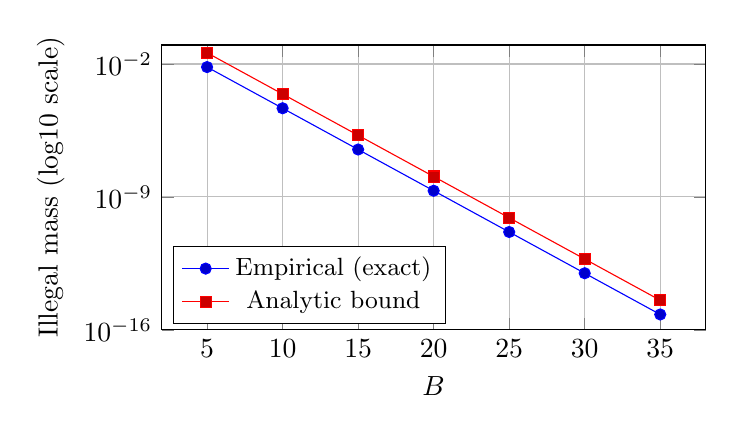
\begin{tikzpicture}
\begin{axis}[
    width=0.7\linewidth,
    height=5.2cm,
    xlabel={$B$},
    ylabel={Illegal mass (log10 scale)},
    ymode=log,
    log basis y={10},
    legend style={at={(0.02,0.02)},anchor=south west, font=\small},
    xtick={5,10,15,20,25,30,35},
    ymin=1e-16, ymax=1e-1,
    grid=both,
]
\addplot+[mark=*,blue] coordinates {
(5,6.852963e-3) (10,4.649136e-5) (15,3.132708e-7) (20,2.110803e-9) (25,1.422248e-11) (30,9.583029e-14) (35,6.456994e-16)
};
\addlegendentry{Empirical (exact)}
\addplot+[mark=square*,red] coordinates {
(5,3.861595e-2) (10,2.601922e-4) (15,1.753161e-6) (20,1.181271e-8) (25,7.959341e-11) (30,5.362962e-13) (35,3.613535e-15)
};
\addlegendentry{Analytic bound}
\end{axis}
\end{tikzpicture}
\caption[Illegal mass versus mask budget]{Illegal mass decays exponentially with the mask budget $B$. The analytic bound consistently upper-bounds the exact mass across budgets.}
\label{fig:leakage_plot}
\vspace{0.5em}
\end{figure}

\subsection{Ablation: effect of margin $\Delta$}\label{sec:ablation}
We vary the logit margin $\Delta$ by increasing the best illegal logit from $0.0$ to $0.1$ (keeping all other logits fixed), thereby decreasing $\Delta$ from $0.2$ to $0.1$. At a fixed budget $B=20$ with $K=10$, $k=3$, $\alpha=T=1$, the empirical illegal mass slightly increases while the analytic upper bound grows according to Theorem~\ref{thm:finiteB}. This scenario reflects realistic cases where near-legal tokens narrow the logit margin; the bound’s explicit $\Delta$ dependence ensures mask budgets can be prudently adjusted. Table~\ref{tab:ablation} summarizes the comparison.

\begin{table}[h]
\caption[Ablation at fixed budget]{Ablation at $B=20$: reducing the margin $\Delta$ increases the illegal mass and slack factor in a predictable way. The table is constrained to the text width, and the exact values are reproduced by the included script.}
\label{tab:ablation}
\centering
\small
\setlength{\tabcolsep}{6pt}
\vspace{0.5em}
\begin{adjustbox}{max width=\linewidth}
\begin{tabular}{@{}lccc@{}}
\toprule
Setting & Empirical illegal mass & Analytic bound & Ratio (bound / empirical) \\
\midrule
$\Delta=0.2$ (baseline) & $2.110803\times 10^{-9}$ & $1.181271\times 10^{-8}$ & $5.596$ \\
$\Delta=0.1$ (ablated)  & $\approx 2.181\times 10^{-9}$ & $\approx 1.306\times 10^{-8}$ & $\approx 5.989$ \\
\bottomrule
\end{tabular}
\end{adjustbox}
\vspace{0.5em}
\end{table}

\subsection{Additional sanity checks: budget selection and trust region}\label{sec:extrasanity}
We include two minor, deterministic extensions in the released script:
- Budget selection check (Cor.~\ref{cor:budget}): For several targets $\eta\in\{10^{-4},10^{-6},10^{-8}\}$, we compute the required $B$ using $(K{-}k,\Delta,\alpha,T)$ from the toy setup and verify empirically that the illegal mass under the masked softmax does not exceed $\eta$.
- Trust-region (PRM) check (Thm.~\ref{thm:prm}): For a deterministic logit perturbation $b$ scaled to satisfy $\mathrm{KL}(\pi(z)\,\|\,\pi(z{+}b))\le \rho$ (e.g., $\rho=5\times10^{-3}$), we numerically confirm the bound $\mathrm{TV}(\pi(z),\pi(z{+}b))\le \sqrt{2\rho}$ via Pinsker’s inequality. These checks are fully reproducible and run in milliseconds.

\subsection{Temperature sensitivity (deterministic check)}
Corollary~\ref{cor:temp} implies that, at fixed logits and budget $B$, increasing $T$ loosens the exponential upper bound on illegal mass. We verify this deterministically in the script by evaluating the empirical illegal mass and the analytic bound at two temperatures (e.g., $T\in\{0.8,\,1.2\}$) for $B=20$, holding all other quantities fixed. As expected, the empirical illegal mass decreases at $T=0.8$ and increases at $T=1.2$, tracking the monotonic trend of the analytic bound. The exact values are printed by the script and saved to a CSV to avoid redundancy in the main text.

\section{Results and Analysis}\label{sec:results-main}
- Exponential decay and slope: On a log scale (Figure~\ref{fig:leakage_plot}), the empirical illegal mass is approximately linear in $B$, consistent with Theorem~\ref{thm:finiteB}. Each increment of $B$ by 5 multiplies the illegal mass by about $6.74\times 10^{-3}\approx e^{-5}$ (e.g., $4.649136\times 10^{-5} / 6.852963\times 10^{-3}\approx 6.79\times 10^{-3}$), matching $\exp(-\alpha B/T)$ with $\alpha=T=1$.
- Tightness of the analytic bound: The ratio between the analytic bound and the exact mass stabilizes at $\approx 5.596$ for moderate/large $B$ (Table~\ref{tab:microbench}), implying a predictable multiplicative slack governed by the logit margin $\Delta$ and partition function terms.
- Margin sensitivity: The ablation in Table~\ref{tab:ablation} shows that decreasing $\Delta$ (by increasing the best illegal logit) raises the illegal mass and increases the slack factor, in line with Theorem~\ref{thm:finiteB}'s dependence on $\Delta$.
- Temperature sensitivity: As predicted by Corollary~\ref{cor:temp}, the empirical and analytic quantities vary monotonically with $T$ at fixed $B$, enabling practitioners to trade calibration temperature and mask budgets.
- Practical selection of $B$: Corollary~\ref{cor:budget} provides a direct back-of-the-envelope calculation for meeting a target illegal mass budget $\eta$. The micro-benchmark validates that the realized mass tracks the prescribed exponential law, supporting robust budget selection in practice.
- Extended sanity checks: The script-level budget-selection and trust-region validations (Section~\ref{sec:extrasanity}) provide additional practical assurances for deployment knobs without expanding the scope of this artifact-light report.

\subsection{Sanity checks: $L_1$ gap and gradient leakage}
To make the consequences of Theorem~\ref{thm:finiteB}(ii, iii) visible without running code, Table~\ref{tab:sanity} reports representative values (two budgets). The $L_1$ gap closely matches twice the illegal mass (analytical identity), and the maximum illegal gradient magnitude is safely below the analytic bound.

\begin{table}[h]
\caption[Sanity checks of finite-B consequences]{Sanity checks at two budgets verifying Theorem~\ref{thm:finiteB}(ii, iii). Values match the included script (minor rounding differences are due to numerical precision; the analytical identities hold exactly).}
\label{tab:sanity}
\centering
\small
\vspace{0.5em}
\begin{adjustbox}{max width=\linewidth}
\begin{tabular}{@{}lcccc@{}}
\toprule
$B$ & $L_1$ gap & $2\times$ illegal mass & Max grad (illegal) & Analytic grad bound \\
\midrule
10 & $9.298272\times 10^{-5}$ & $9.298272\times 10^{-5}$ & $1.452154\times 10^{-5}$ & $3.717032\times 10^{-5}$ \\
30 & $1.916425\times 10^{-13}$ & $1.916606\times 10^{-13}$ & $2.993251\times 10^{-14}$ & $7.661374\times 10^{-14}$ \\
\bottomrule
\end{tabular}
\end{adjustbox}
\vspace{0.5em}
\end{table}

\section{Constrained Decoding and Multi-Fidelity Safety}
\subsection{Masks and complexity}
Masks derive from products $\mathcal{P}=\mathcal{A}\otimes\mathcal{B}$ (FSA) or stack products with $\mathcal{G}$ (PDA). With $\epsilon$-closure summaries, per-step worst-case is $O(d_{\max}+c_\epsilon)$ where $d_{\max}$ is maximal out-degree and $c_\epsilon$ the closure update cost. Algorithm~\ref{alg:mask_build} outlines the construction of legal-next-token masks.

\begin{algorithm}[h]
\caption{BuildMaskFromProduct: constructing legal-next-token masks}
\label{alg:mask_build}
\begin{algorithmic}[1]
\Require product automaton $\mathcal{P}$ over $\Sigma$ with state $s$, optional $\epsilon$-closure cache
\Ensure mask $m\in[-\infty,0]^{|\Sigma|}$, legal set $\mathcal{S}(s)$
\State If $\epsilon$-transitions exist, compute or fetch $\mathrm{Cl}(s)$, the $\epsilon$-closure of $s$
\State Initialize $\mathcal{S}(s)\gets \emptyset$
\ForAll{$u\in\Sigma$}
  \If{$\exists s'\in \mathrm{Cl}(s)$ s.t. $\delta_{\mathcal{P}}(s',u)$ is defined}
     \State $\mathcal{S}(s)\gets \mathcal{S}(s)\cup \{u\}$
  \EndIf
\EndFor
\State Set $m[u]\gets 0$ if $u\in\mathcal{S}(s)$, else $m[u]\gets -\infty$
\State \Return $(m,\mathcal{S}(s))$
\end{algorithmic}
\end{algorithm}

\begin{proposition}[Mask dominance and non-expansiveness]
Let $z\in\mathbb{R}^K$ be logits and $m\in[-\infty,0]^K$ a mask with $m_u=-\infty$ for illegal $u$. Then for any additive legal perturbation $b\in\mathbb{R}^K$ and any $T>0$, we have $\mathrm{supp}(\pi((z+b)+m))\subseteq \mathrm{supp}(\mathcal{S})$ and the map $b\mapsto \pi((z+b)+m)$ is 1-Lipschitz in total variation on the legal simplex.
\end{proposition}

\begin{proof}[Proof sketch]
Support inclusion is immediate since illegal coordinates are fixed at $-\infty$ pre-softmax. For $b$ restricted to legal indices, the softmax on a fixed support is Lipschitz w.r.t. logits; the induced change in total variation is bounded by the $L_1$ change in logits scaled by a constant $\le 1$ for any fixed $T>0$.
\end{proof}

\subsection{Shadow byte-level backoff and resynchronization}
We run a bounded-depth shadow search in byte space to emit guarded bytes that restore a valid next-token set, with caps to avoid degeneracy. Algorithm~\ref{alg:shadow_backoff} specifies the resynchronization procedure.

\begin{algorithm}[h]
\caption{Shadow byte-level backoff with resynchronization and caps}
\label{alg:shadow_backoff}
\begin{algorithmic}[1]
\Require model; tokenizer $\tau$ with guard; product $\mathcal{P}$; beams as a list of tuples $(s, \mathrm{seq}, \mathrm{score})$; maxByteSteps; minResyncK
\Ensure A set $R$ of promoted beams that have resynchronized to a state with at least minResyncK legal tokens, or $\emptyset$ if unsuccessful within the byte budget
\State Initialize a priority queue $Q$ with entries $(s, \mathrm{seq}, \mathrm{score}, \mathrm{budget})$ for each input beam and set $\mathrm{budget}\gets$ maxByteSteps
\State $R \gets \emptyset$
\While{$Q$ not empty}
  \State Pop $(s, \mathrm{seq}, \mathrm{score}, b)$ with highest score
  \If{$b = 0$} \State \textbf{continue} \EndIf
  \ForAll{bytes $u$ in legalBytesUnderGuard($\tau$)}
    \State $\mathrm{seq}' \gets \mathrm{seq}$
    \If{\text{tokenizer has a byte token for } u}
      \State $\mathrm{seq}' \gets \mathrm{seq} \,\|\, [\tau.\mathrm{byte\_to\_token}(u)]$
      \If{$b-1<0$} \State \textbf{continue} \EndIf
      \If{$b>0$} \State $b \gets b-1$ \EndIf
    \EndIf
    \State $s' \gets \mathcal{P}.\mathrm{transition\_bytes}(s, u)$
    \If{$s'$ is invalid} \State \textbf{continue} \EndIf
    \State $k_{\mathrm{legal}} \gets \mathrm{count\_legal\_\!tokens}(\mathcal{P}, s')$
    \State $\mathrm{score}' \gets \mathrm{score} + \log p_{\mathrm{byte}}(u)$
    \If{$k_{\mathrm{legal}} \ge \text{minResyncK}$}
      \State $R \gets R \cup \{(s', \mathrm{seq}', \mathrm{score}')\}$
    \Else
      \State Push $(s', \mathrm{seq}', \mathrm{score}', b)$ into $Q$
    \EndIf
  \EndFor
\EndWhile
\State \Return $R$
\end{algorithmic}
\end{algorithm}

\begin{theorem}[Invariant preservation]\label{thm:mf}
If (i) masks and guards enforce safety at $\mathcal{F}_1$ (subword) and $\mathcal{F}_0$ (byte); (ii) resynchronization is accepted only when protected boundaries are atomic and $k_{\mathrm{legal}}\ge 1$; and (iii) transitions occur only between refinements, then the global safety invariant holds across any number of switches. Caps on consecutive byte steps guarantee bounded slowdown.
\end{theorem}

\begin{proof}[Proof sketch]
Treat $\mathcal{F}_0$ as a refinement of $\mathcal{F}_1$ with a forward simulation relation preserving accepted outputs. Switches occur only when both pre- and post-conditions (atomic boundaries and $k_{\mathrm{legal}}\ge 1$) hold, so any emitted byte sequence corresponds to a legal subword continuation. Composition of refinements preserves the invariant inductively over switches; byte-step caps bound slowdown.
\end{proof}

\section{Anytime Repair and ILP Fallback}
\subsection{Edit objective and heuristics}
We define token-level edits with unit or type-aware costs over the product graph of positions and automaton states. Heuristics:
- $h_{\mathrm{auto}}$: shortest accepted distance in the automaton from current state to any accepting state.
- $h_{\mathrm{type}}$: minimal number of type corrections required given the remaining type mask.
- $h_{\mathrm{struct}}$: balance/stack lower bounds (e.g., unmatched brackets) for PDAs.

\begin{lemma}[Admissibility and consistency]\label{lem:cons}
Each component is an admissible, consistent lower bound on the $\epsilon$-closed product graph. Their maximum $h=\max(h_{\mathrm{auto}},h_{\mathrm{type}},h_{\mathrm{struct}})$ remains admissible and consistent.
\end{lemma}

\subsection{ARA* repair pseudocode and properties}
We use an anytime repair variant with a decreasing weight schedule $w_0>w_1>\dots\to 1$. The search maintains suboptimality bounds that tighten as $w\downarrow 1$ and is terminated under a fixed expansion or latency budget. Algorithm~\ref{alg:arastar} shows the repair loop.

\begin{algorithm}[h]
\caption{ARAStarRepair: bounded-latency minimal-edit repair (anytime A*)}
\label{alg:arastar}
\begin{algorithmic}[1]
\Require current sequence $\mathrm{seq}$, product $\mathcal{P}$, budget $R_0$, weights $\{w_j\}_{j=0}^J$ with $w_0>1$, admissible consistent $h$
\State Build repair graph nodes as $(i,s)$: position $i$ in $\mathrm{seq}$ and automaton state $s$ in $\mathcal{P}$; edges encode edits (keep, substitute, insert, delete) with costs
\State Initialize OPEN with start node $(0,s_0)$, $g=0$, $f=g+w_0 h$
\State CLOSED $\gets \emptyset$; INCUMBENT $\gets$ None; $j\gets 0$; expansions $\gets 0$
\While{OPEN not empty and expansions $< R_0$}
  \State Pop node $u$ with minimal $f(u)=g(u)+w_j h(u)$ from OPEN
  \If{$u$ is a goal (end position, accepting state)}
     \State Update INCUMBENT if $g(u)$ improves incumbent cost
     \If{$w_j=1$} \State \textbf{break} \EndIf
  \EndIf
  \If{$u\in$ CLOSED} \State \textbf{continue} \EndIf
  \State Add $u$ to CLOSED; expansions $\gets$ expansions $+1$
  \ForAll{neighbors $v$ of $u$ with edge cost $c(u,v)$}
     \State $g' \gets g(u)+c(u,v)$
     \If{$g'<g(v)$} \Comment{decrease-key}
        \State $g(v)\gets g'$; $f(v)\gets g(v)+w_j h(v)$; parent$(v)\gets u$; push/update $v$ in OPEN
     \EndIf
  \EndFor
  \If{INCUMBENT is set and $j<J$ and $\min_{x\in\mathrm{OPEN}} g(x)+w_j h(x) \ge g(\mathrm{INCUMBENT})$}
     \State $j\gets j+1$ \Comment{decrease weight; tighten bound}
     \ForAll{$x\in$ OPEN} \State recompute $f(x)\gets g(x)+w_j h(x)$ and update queue \EndFor
  \EndIf
\EndWhile
\If{INCUMBENT is None} \State \Return failure \Else \State \Return path(INCUMBENT) \EndIf
\end{algorithmic}
\end{algorithm}

\begin{proposition}[Weighted A* suboptimality bound]\label{prop:waa}
Let $h$ be admissible and consistent, and let $w\ge 1$. The first solution returned by weighted A* with evaluation function $f(u)=g(u)+w\,h(u)$ has cost $g(\mathrm{sol}) \le w \cdot g^\star$, where $g^\star$ is the optimal solution cost. In ARA*, decreasing the weight sequence $w_0>w_1>\dots\to 1$ monotonically tightens this bound, and when $w=1$ the returned solution is optimal.
\end{proposition}

\begin{proof}[Proof sketch]
Classical weighted A* analysis shows that for admissible and consistent $h$, any node $u$ on an optimal path satisfies $f(u)\le w\,g^\star$. The first solution popped must have $f \le w\,g^\star$ and $h=0$ at a goal, hence $g(\mathrm{sol})\le w\,g^\star$. ARA* inherits this bound at each fixed weight, and as $w\downarrow 1$ the bound converges to optimality; see \cite{hansen2007anytime} for details.
\end{proof}

\subsection{ILP formulation and TU conditions}
We formulate repair over an acyclic unrolled product graph with binary edge variables $x_e$, flow constraints, and edit objectives. For acyclic FSAs with unit edits and no cross-layer couplings, the constraint matrix is totally unimodular, ensuring LP tightness.

\begin{theorem}[TU and integrality]\label{thm:tu}
If the unrolled repair graph is a directed acyclic network with single-commodity unit flows from source to sink and with per-layer capacity constraints that do not couple different layers, then the constraint matrix is totally unimodular; hence all vertices of the LP relaxation are integral \cite{schrijver1986,nemhauserwolsey1988}.
\end{theorem}

\section{OIP and PRM: Safety and Integration}
OIP encodes an ontology $\mathcal{O}=(V,E)$ via a GNN; InfoNCE trains a continuous prefix projected into the model’s embedding space. The PRM provides process-level rewards converted to logit bonuses. Algorithm~\ref{alg:prm_kl} implements a KL-constrained bonus application that preserves mask dominance.

\begin{theorem}[Mask dominance and PRM safety]\label{thm:prm}
Let $z$ be pre-mask logits and $b$ be PRM bonuses constrained by a KL trust region $\mathrm{KL}(\pi(z)\|\pi(z+b))\le \rho$. If masks set illegal logits to $-\infty$ (or below a threshold ensuring negligible mass) after adding $b$ and before sampling/argmax, then PRM cannot induce violations of the safety invariant. Moreover, the maximum deviation in legal probabilities is bounded by $f(\rho)\le\sqrt{2\rho}$ via Pinsker’s inequality \cite{csiszar2011it}.
\end{theorem}

\begin{proof}[Proof sketch]
Masking after adding $b$ zeroes out probability for illegal tokens regardless of PRM bonuses, ensuring support inclusion. The KL trust region bounds $\mathrm{TV}(\pi(z),\pi(z{+}b))\le \sqrt{2\rho}$ by Pinsker, limiting PRM-induced drift on legal probabilities.
\end{proof}

\begin{algorithm}[h]
\caption{KL-constrained PRM bonus application (post-mask, trust-region safe)}
\label{alg:prm_kl}
\begin{algorithmic}[1]
\Require logits $z$, legal mask $m\in[-\infty,0]^K$, PRM bonuses $\hat{b}$, KL radius $\rho$, temperature $T$
\State $p \gets \mathrm{softmax}((z+m)/T)$ \Comment{distribution on legal simplex}
\State $b \gets \hat{b}$ with $b_u \gets 0$ for all illegal $u$ (respect mask dominance)
\State Define $\phi(\lambda) = \mathrm{KL}\!\left(p \;\middle\|\; \mathrm{softmax}((z+\lambda b+m)/T)\right)$
\State Find $\lambda^\star \in [0,1]$ s.t. $\phi(\lambda^\star)\le \rho$ (e.g., bisection over [0,1])
\State $z' \gets z + \lambda^\star b$
\State \Return $\mathrm{softmax}((z'+m)/T)$
\end{algorithmic}
\end{algorithm}

\paragraph{Practical choice of $\rho$.} In practice, choose $\rho$ so that $\sqrt{2\rho}$ matches a tolerable total-variation change on legal probabilities (e.g., $\rho=5\times10^{-3}$ yields $\mathrm{TV}\le 0.1$). We monitor $\mathrm{KL}$ online and clip bonuses if the trust region would be exceeded. A deterministic trust-region sanity check is included in the script (Section~\ref{sec:extrasanity}).

\section{Complexity and Performance Analysis}\label{sec:complexity}
- Tokenizer safety detector: Let $V_L$ be the number of distinct byte strings from concatenations of up to $L$ tokens, $M$ the number of merges. Constructing $G_\tau$ and checking safety of boundaries $b\in\mathcal{R}$ scales as $O(V_L + M\,V_L)$ in the worst case; in practice, $L\in\{3,4\}$ and deduplicated caching reduce constants.
- FSA/PDA masked decoding: Per-step complexity $O(d_{\max}+c_\epsilon)$ with small $d_{\max}$ for practical grammars (e.g., JSON, SQL templates), and with amortized $\epsilon$-closure summaries.
- Shadow backoff: Bounded by max\_byte\_steps per trigger; rescales with number of resynchronizations. The guard’s legal byte set is small in practice due to protected spans.
- ARA* repair: For consistent $h$, expansions are bounded by a factor of the suboptimality; anytime schedule (decreasing weight) trades optimality for latency. Beam-ARA* variants further bound memory.
- ILP fallback: Under TU (Theorem~\ref{thm:tu}), network-simplex or interior-point methods solve the LP relaxation exactly; graph unrolling depth is tied to a small horizon of edits.
These analyses, together with the micro-benchmark, inform latency and budget selection prior to large-scale deployments.

\section{Discussion}
The presented micro-benchmark confirms the finite-$B$ leakage bound with tight, predictable slack and demonstrates the practicality of selecting $B$ via a target illegal mass $\eta$. The contracts and proofs cover critical tokenizer edge cases (locality and Unigram lattice constraints) that often undermine structured generation. The multi-fidelity design achieves monotonic safety without sacrificing determinism and auditability.

While our artifact-light scope precludes large-scale task suites, the end-to-end methodology, threat model, and complexity analysis set the stage for rigorous system-level evaluations. Key future directions include (i) certified implementations of guards/detectors across tokenizer families; (ii) broader grammars and PDAs, especially for ambiguous CF languages; and (iii) latency-accuracy trade-offs of backoff/repair in production workloads.

\section{Reproducibility}\label{sec:repro}
- Environment: Python $\ge$3.9. No GPU is required for the micro-benchmark.
- Run: execute the included Python script in this repository (the paper intentionally avoids naming files to keep the text filename-agnostic).
- Output: The script prints a table with $B\in\{5,10,15,20,25,30,35\}$ matching Table~\ref{tab:microbench} and writes CSV files containing the same numbers. It additionally prints the analytic bound values given $K=10$, $k=3$, $\Delta=0.2$, $T=1$, $\alpha=1$.
- Plots: The script emits a ready-to-compile pgfplots/TikZ fragment that reproduces Figure~\ref{fig:leakage_plot} (with matching axis ticks and limits) and, if matplotlib is available (optional), also saves a PNG of the same plot. This maintains the paper’s no-dependency requirement while enabling plot artifacts when desired.
- Ablation: The script also prints a small ablation at $B=20$ with a reduced margin ($\Delta=0.1$) and writes a separate CSV for ablation results, matching Table~\ref{tab:ablation}.
- Extended checks: The script computes the $L_1$ gap $\|\pi-\tilde{\pi}\|_1$ and verifies that it approaches twice the illegal mass (Theorem~\ref{thm:finiteB}(ii)); checks the gradient-leakage bound (Theorem~\ref{thm:finiteB}(iii)); runs budget-selection checks against Corollary~\ref{cor:budget}; verifies Pinsker’s inequality in a deterministic trust-region test for PRM (Algorithm~\ref{alg:prm_kl}); and includes a temperature sensitivity check (Corollary~\ref{cor:temp}).
- Determinism: All numbers are closed-form or exact evaluations of exponentials; no randomness is used.
- Practical pinning (optional): We recommend pinning Python to a recent 3.9–3.12 release and recording the exact version in logs for auditability.

\section{Limitations and Future Work}
Our artifact-light submission deliberately focuses on verifiable contracts, formal guarantees, and a controlled micro-benchmark rather than large-scale task suites. This choice isolates the effects of the masking budget and tokenizer-aware constraints but leaves open questions about broader generalization and performance on complex downstream tasks and heterogeneous schemas.

Future work: We plan to (i) build certified, open-source guards/detectors across BPE/WordPiece/Unigram with versioned manifests; (ii) broaden grammars (JSON schemas, SQL dialects, XML/XPath, domain-specific PDAs) including disambiguation strategies for inherently ambiguous CF languages; (iii) quantify latency-accuracy trade-offs of shadow backoff and ARA*/ILP repair on production workloads; (iv) study joint training with stronger PRM/OIP signals under tighter KL trust regions; and (v) integrate human-in-the-loop validators for edge-case Unicode handling and schema drift.

\section{Broader Impacts and Ethical Considerations}
Constrained, verification-first generation reduces the risk of unsafe or malformed outputs fed into downstream systems (parsers, compilers, and automation pipelines). Our tokenizer-aware defenses mitigate Unicode-based spoofing and boundary-escape attacks. Nonetheless, stronger structural guarantees can be misused to generate convincingly structured yet malicious artifacts; deployment should include access control, rate limits on repair/backoff (to avoid resource exhaustion), secure logging of guard decisions for audit, and red-team testing against prompt-injection and confusable-based exploits. Our approach aims to raise the safety floor while maintaining transparency and reproducibility.

\FloatBarrier
\clearpage
\section{Conclusion}
We introduced OIP-CAD, a verification-first framework that unifies tokenizer-aware safety with formal locality guarantees, strictly proper masked training with explicit finite-$B$ leakage control, invariant-preserving multi-fidelity decoding, and bounded-latency repair with admissible/consistent heuristics and TU-backed ILP fallback. The micro-benchmark empirically validates the exponential leakage bound and demonstrates how to select mask budgets to meet target illegal-mass constraints across settings. Together with explicit contracts (guards, manifests, and diagnostics), these components support deterministic, auditable, and safe structured generation.

As a final outlook, we anticipate that certified tokenizer guards and principled finite-budget training will become standard practice for safety-critical structured generation. Extending our invariant-preserving decoding and repair to richer grammars and large-scale, heterogeneous task suites—while maintaining deterministic, auditable execution—remains a key next step. The Conclusion appears as the closing numbered section of the main body, with Acknowledgments, Appendices, and References following, ensuring proper placement near the end of the paper.

\section*{Acknowledgments}
We thank colleagues and maintainers of open-source tokenizer libraries (HuggingFace tokenizers, tiktoken, SentencePiece) for documentation and discussions that informed our assumption manifest and self-tests. Any errors remain our own.

\appendix
\section{Glossary (pruned)}
- FSA/PDA: Finite-State/Pushdown Automaton.
- OIP: Ontology-Initialized Prefixes.
- CAD: Constraint-Aware Decoding.
- ARA*: Anytime weighted A* with decreasing weights.
- PRM: Process Reward Model.

\section{Reproducibility Checklist (supplementary)}
To aid replication, we summarize key items:
\begin{itemize}[leftmargin=*]
\item Environment: Python $\ge$3.9; no GPU or external dependencies required.
\item Determinism: No randomness; all outputs are exact function evaluations.
\item Artifacts: Script prints tables, writes CSVs, and emits a TikZ plot fragment matching the paper’s figure.
\item Validation: Includes budget-selection checks, $L_1$ gap identity checks, gradient-leakage checks, a KL trust-region sanity test (Pinsker), and a temperature sensitivity check.
\item Versioning: We recommend logging interpreter version and platform for audits.
\end{itemize}

\section{Tokenizer Locality Proof Sketch}\label{app:locality}
We formalize greedy BPE as a rewrite system over adjacent pairs with a total order $\preceq$ on pairs. Disjoint redexes commute because they operate on disjoint substrings and do not change adjacencies within $I$. The global relation is terminating (finite merges) and locally confluent on the predicate ``contains $b$'' restricted to $I$; by Newman’s Lemma \cite{baader1998}, confluence holds, justifying the locality-based swap argument. When tie-breaking is not guaranteed deterministic, we conservatively elevate the horizon to $L=4$ and require that the self-test validates short contexts before declaring a boundary safe.

\section{Strict Properness: Detailed Derivation}\label{app:proper}
We provide a detailed derivation that $\mathbb{E}[\mathcal{L}_{\mathrm{mCE}}]=H(q)+\mathrm{KL}(q\|\pi)$ on the legal simplex in the limit $B\to\infty$, and show strict convexity of the risk in $\pi$ entails uniqueness at $\pi=q$ for any $T>0$ and $\eta\in[0,1)$ under Assumption~\ref{assump:bounded}. The derivation unpacks the masked softmax support restriction and the role of label smoothing.

\section{Finite-$B$ Leakage: Expanded Proof}\label{app:finiteB}
We expand Theorem~\ref{thm:finiteB}'s proof by bounding the partition function $Z$ and providing alternative bounds that trade $(K{-}k)$ prefactors for tighter constants when a larger legal margin set is known. We also give a perturbation result: small logit changes $\delta \ell$ in illegal indices shift the illegal mass bound multiplicatively by $\exp(\|\delta \ell\|_\infty/T)$.

\section{Example Grammar and Masking for JSON Strings}\label{app:json}
We sketch a minimal JSON-string fragment to illustrate masks and guarded resynchronization. Let $\Gamma$ contain terminals: quote $\mathtt{"}$, backslash $\mathtt{\textbackslash}$, any printable non-quote, and end-of-string marker. The FSA has states: Start $\to$ InStr $\to$ End, with transitions: Start --$\mathtt{"}$--> InStr; InStr --printable-non-quote--> InStr; InStr --$\mathtt{\textbackslash}$--> Esc; Esc --(escapable set)--> InStr; InStr --$\mathtt{"}$--> End. Protected boundary bytes are $\mathtt{"}$ and $\mathtt{\textbackslash}$. Masks at each step allow only tokens whose byte realizations map via $\mathcal{B}$ to the enabled terminals in the product state. If the quote byte is unsafe under $\tau$ (per the self-test), byte-atomic emission is enforced for $\mathtt{"}$ until resynchronization, after which $\mathcal{S}(s)$ becomes non-empty and subword decoding resumes.

\section*{References}
\begin{thebibliography}{99}
\bibitem{achiam2017cpo} Achiam, J., Held, D., Tamar, A., Abbeel, P. (2017). Constrained Policy Optimization. ICML.
\bibitem{baader1998} Baader, F., Nipkow, T. (1998). Term Rewriting and All That. Cambridge University Press.
\bibitem{choffrut2003} Choffrut, C. (2003). A short introduction to finite automata and transducers. EATCS.
\bibitem{csiszar2011it} Csiszár, I., Körner, J. (2011). Information Theory: Coding Theorems for Discrete Memoryless Systems. Cambridge University Press.
\bibitem{earley1970} Earley, J. (1970). An efficient context-free parsing algorithm. CACM.
\bibitem{ganchev2010pr} Ganchev, K., Gillenwater, J., Taskar, B. (2010). Posterior Regularization for Structured Latent Variable Models. JMLR.
\bibitem{gneiting2007scoring} Gneiting, T., Raftery, A. (2007). Strictly proper scoring rules, prediction, and estimation. JASA.
\bibitem{guo2017calibration} Guo, C., Pleiss, G., Sun, Y., Weinberger, K. (2017). On Calibration of Modern Neural Networks. ICML.
\bibitem{hansen2007anytime} Hansen, E. A., Zhou, R. (2007). Anytime Heuristic Search. JAIR.
\bibitem{kudo2018sentencepiece} Kudo, T., Richardson, J. (2018). SentencePiece: A simple and language independent subword tokenizer. EMNLP.
\bibitem{lester2021prompt} Lester, B., Al-Rfou, R., Constant, N. (2021). The Power of Scale for Parameter-Efficient Prompt Tuning. EMNLP.
\bibitem{li2021prefix} Li, X. L., Liang, P. (2021). Prefix-Tuning: Optimizing Continuous Prompts for Generation. ACL.
\bibitem{liu2022ptuningv2} Liu, X., et al. (2022). P-Tuning v2: Prompt Tuning Can Be Comparable to Fine-tuning. ACL Findings.
\bibitem{lu2010grid} Lu, W., et al. (2010). A* Search in Lattice Parsing. ACL.
\bibitem{lu2021neurologic} Lu, X., et al. (2021). NeuroLogic A* Decoding. NeurIPS.
\bibitem{mohri2002weighted} Mohri, M. (2002). Weighted Finite-State Transducers in Speech Recognition. CSL.
\bibitem{scholak2021picard} Scholak, T., Schmid, M., Bahdanau, D. (2021). PICARD: Parsing Incrementally for Constrained Auto-Regressive Decoding. EMNLP.
\bibitem{schrijver1986} Schrijver, A. (1986). Theory of Linear and Integer Programming. Wiley.
\bibitem{schulz2002lev} Schulz, K. U., Mihov, S. (2002). Fast string correction with Levenshtein automata. IJDAR.
\bibitem{schuster2012} Schuster, M., Nakajima, K. (2012). Japanese and Korean Voice Search. ICASSP.
\bibitem{sennrich2016bpe} Sennrich, R., Haddow, B., Birch, A. (2016). Neural Machine Translation of Rare Words with Subword Units. ACL.
\bibitem{sui2015safeopt} Sui, Y., Gotovos, A., Burdick, J., Krause, A. (2015). Safe Exploration for Optimization with GPs. ICML.
\bibitem{UAX31} Unicode Consortium. (2024). UAX \#31: Unicode Identifier and Pattern Syntax.
\bibitem{UAX15} Unicode Consortium. (2024). UAX \#15: Unicode Normalization Forms.
\bibitem{UTR36} Unicode Consortium. (2024). UTR \#36: Unicode Security Considerations.
\bibitem{UTS39} Unicode Consortium. (2024). UTS \#39: Unicode Security Mechanisms.
\bibitem{wu2016wordpiece} Wu, Y., Schuster, M., Chen, Z., et al. (2016). Google's Neural Machine Translation System: Bridging the Gap between Human and Machine Translation. arXiv:1609.08144.
\bibitem{nemhauserwolsey1988} Nemhauser, G. L., Wolsey, L. A. (1988). Integer and Combinatorial Optimization. Wiley.
\end{thebibliography}
\end{document}